\documentclass[12pt]{beamer}
%\documentclass[handout,xcolor=pdflatex,dvipsnames,table,12pt]{beamer}
\usepackage[latin1]{inputenc}
%\usepackage[T1]{fontenc}
\usepackage{amsmath} % for math AMS fonts
\usepackage{graphicx} % to include figures
\usepackage{subfigure} % to have figures in figures
\usepackage{multimedia} % to include movies
\usepackage{listings} % to display code
\usepackage{colortbl} % colored tables
\usepackage[latin1]{inputenc} % support for accented letters, etc.
\usepackage{amsthm}
\usepackage{hyperref}
\usepackage{ulem}
\usepackage{booktabs}

\usetheme{Warsaw}
\setbeamercovered{transparent}

\title[Introduction to Cryptography]{Quantum Computation and Cryptography}
\author{Christian Mann -- christian-mann@utulsa.edu}
\institute{University of Tulsa\\
Tulsa, Oklahoma 74104}
\date{\today}

\logo{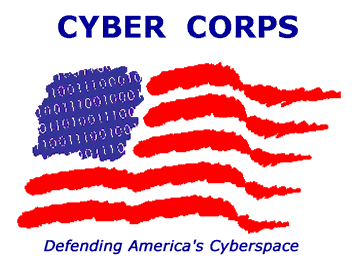
\includegraphics[height=1.5cm]{pictures/SFSLogoMain}}

\begin{document}

\lstset{
language=python,                % choose the language of the code
%basicstyle=\footnotesize,       % the size of the fonts that are used for the code
%numbers=left,                   % where to put the line-numbers
%numberstyle=\footnotesize,      % the size of the fonts that are used for the line-numbers
%stepnumber=2,                   % the step between two line-numbers. If it's 1 each line will be numbered
%%umbersep=5pt,                  % how far the line-numbers are from the code
%backgroundcolor=\color{white},  % choose the background color. You must add \usepackage{color}
showspaces=false,               % show spaces adding particular underscores
showstringspaces=false,         % underline spaces within strings
showtabs=false,                 % show tabs within strings adding particular underscores
%%frame=single,	                % adds a frame around the code
tabsize=4,	                % sets default tabsize to 2 spaces
%%captionpos=b,                   % sets the caption-position to bottom
%%breaklines=true,                % sets automatic line breaking
%%breakatwhitespace=false,        % sets if automatic breaks should only happen at whitespace
%%title=\lstname,                 % show the filename of files included with \lstinputlisting; also try caption instead of title
%escapeinside={\%*}{*)}          % if you want to add a comment within your code
%morekeywords={*,...}            % if you want to add more keywords to the set
}

\newtheorem{mydef}{Definition}

\newcommand{\ket}[1]{\ensuremath{|#1\rangle}}


\begin{frame}
\titlepage
\end{frame}


% no outline

% note, you should have three sections maximum.  two is good.  subsubsections are evil.
% new slides begin with teh \begin{frame} and end with \end{frame}

\iffalse
Quantum Physics: Superposition and Entanglement
Quantum Computing - Theoretical Model?
Shor's Algorithm
Grover's Algorithm
Quantum Annealing
Post-Quantum Cryptography
Quantum Error Correction?
\fi

\begin{frame}{Quantum Physics}{``If you think you understand quantum mechanics...
	you don't understand quantum mechanics'' -- Feynman}

	\begin{block}{Superposition}
		A quantum system can be in a multitude of states at once, according to a
		probability distribution
	\end{block}

	\begin{block}{Entanglement}
		Different parts of a quantum system can be connected such that changes
		to one particle are reflected in the other, connected particle.
	\end{block}

	\begin{alertblock}{What this does not mean}
		Instantaneous communication. An outsider cannot influence the
		information being transmitted.
	\end{alertblock}
\end{frame}

\begin{frame}{Quantum Physics}
	\begin{block}{Qubit}
		A \textbf{qubit}, or quantum bit, is a unit of quantum information.
		Usually some two-state system, a qubit is capable of being in ``two
		states at once'' via superposition.

		When measured, the qubit will collapse into a single state.
	\end{block}

	To talk about qubits, there needs to be a set of basis vectors. We use the
	computational basis of \ket0 and \ket1.
\end{frame}

\begin{frame}{Qubits}
	\begin{block}{State of a qubit}
		A qubit is in a linear superposition of the basis states, so its state
		can be represented as a linear combination of \ket0 and \ket1:
		\[ \ket{\Psi} = \alpha\ket0 + \beta\ket1 \]
		Each of $\alpha$ and $\beta$ are complex numbers.
	\end{block}
	
	\begin{block}{Measuring a qubit}
		When we measure a qubit in the standard basis, the probability of
		outcome $\ket0$ is $|\alpha|^2$ and of $\ket1$ is $|\beta|^2$. Therefore
		it must be that
		\[ |\alpha|^2 + |\beta|^2 = 1 \]
	\end{block}
\end{frame}

\begin{frame}{Qubits}
	\begin{block}{Qubit entanglement}
		Multiple qubits can exhibit quantum entanglement, meaning the
		\textit{entire system} can be in a well-defined state of superposition.

		\[ \ket\Psi = \frac{1}{\sqrt2}(\ket{00} + \ket{11}) \]

		There is an equal probability of measuring either $\ket{00}$ or
		$\ket{11}$, and zero probability of measuring either $\ket{01}$ or
		$\ket{10}$.
	\end{block}
\end{frame}

\begin{frame}{Qubits}
	There are many proposed materials to create qubits from. Each has its
	strengths and weaknesses, primarily involving error rate.
	\begin{block}{Qubit Materials}
		\begin{itemize}
		\item Photon polarization
		\item Electron spin
		\item Electron number (charge)
		\item Nuclear spin
		\item Quantum dot spin
		\end{itemize}
	\end{block}
\end{frame}

\begin{frame}{Quantum Algorithms}{Without a Ph.D. in Physics}
	\begin{block}{Quantum Logic Gate}
		There are certain atomic operations possible to be performed on
		collections of qubits. Particularly, operations are unitary
		transformations, meaning they preserve $\sum |\alpha_i|^2$.
	\end{block}

	\[ v_0\ket0 + v_1\ket1 \rightarrow \left[ \begin{array}{c} v_0 \\ v_1
	\end{array} \right] \]

	\[ v_{00}\ket{00} + v_{01}\ket{01} + v_{10}\ket{10} + v_{11}\ket{11}
	\rightarrow
	\left[ \begin{array}{c} v_{00} \\ v_{01} \\ v_{10} \\ v_{11} \end{array} \right] \]
\end{frame}

\begin{frame}{Quantum Algorithms}{Some Gates}
	\[ X = NOT = \left[ \begin{array}{cc} 0 & 1 \\ 1 & 0 \end{array} \right] \]
	
	\[ SWAP = \left[ \begin{array}{cccc}
		1 & 0 & 0 & 0 \\
		0 & 0 & 1 & 0 \\
		0 & 1 & 0 & 0 \\
		0 & 0 & 0 & 1
	\end{array} \right] \]

	\[ \sqrt{SWAP} = \left[ \begin{array}{cccc}
		1 & 0 & 0 & 0 \\
		0 & \frac{1}{2}(1+i) & \frac{1}{2}(1-i) & 0 \\
		0 & \frac{1}{2}(1-i) & \frac{1}{2}(1+i) & 0 \\
		0 & 0 & 0 & 1
	\end{array} \right] \]
\end{frame}

\begin{frame}{Quantum Computation}
	\begin{block}{Probabilistic Computing}
		Generally quantum algorithms do not guarantee the right answer (state); they
		merely make it more \textbf{likely} than all wrong answers.

		Usually this is fine; we just re-run the algorithm until it gives us a
		useful answer.
	\end{block}

	\begin{block}{}
		The general idea is that we start with qubits in a certain state, and
		apply operators (gates) to groups of qubits, to make the invalid states
		destructively interfere, while the correct solutions constructively
		interfere.
	\end{block}
\end{frame}

\begin{frame}{Quantum Computation}
	\begin{block}{Quantum Algorithm Paradigms}
		\begin{itemize}
			\item Quantum Circuit (Gate Array)
			\item Adiabatic Quantum Computer
			\item Topological Quantum Computer
			\item There are others
		\end{itemize}
	\end{block}
	Each of these can simulate the others with little overhead.
\end{frame}

\begin{frame}{Quantum Error Rate}
	In practice, the area of greatest research is quantum error detection,
	prevention, and correction. Qubits turn out to not want to hold their values
	for more than a few seconds at a time.
\end{frame}

\begin{frame}{Existing Quantum Computers}
	Quantum computers can be simulated by a classical computer with exponential
	effort.

	D-Wave has built multiple adiabatic quantum computers; can be used to solve
	optimizations. It has about 512 qubits. No evidence of quantum speedup has
	been shown.
\end{frame}

\begin{frame}{Shor's Algorithm}
	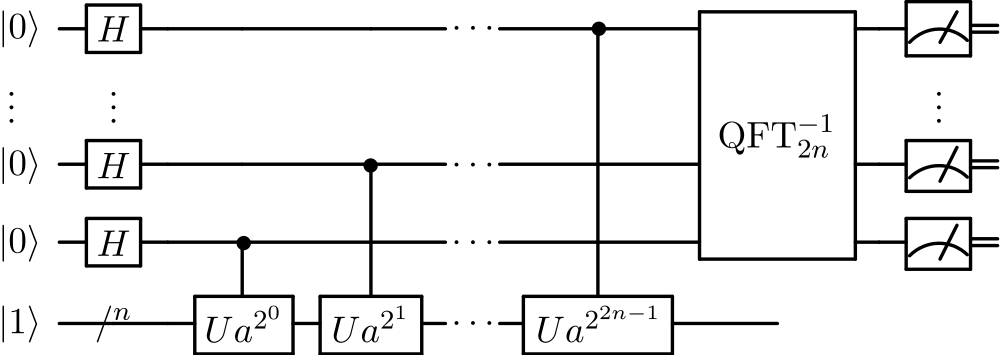
\includegraphics[width=\framewidth]{pictures/shor}
\end{frame}

\begin{frame}{Shor's Algorithm}
	\begin{itemize}
		\item Factorization algorithm
		\item Requires around $2 * \log N$ qubits
		\item $O((\log N)^2(\log\log N)(\log\log\log N))$
		\item Previous best: GNFS -- about $O(e^{1.9 (log N)^{1/3}(\log
			N)^{2/3}})$, sub-exponential but still not polynomial
	\end{itemize}
	Largest number factored so far was until recently 21; as of Nov
	2014 the largest factored was $56153 = 223 x 241$. \textit{Note:}
	only possible due to information already known about factors.
	\begin{alertblock}{}
		This algorithm also works for elliptic curve groups, and requires way
		fewer qubits.
	\end{alertblock}
\end{frame}

\begin{frame}{Shor's Algorithm}
	\begin{block}{Discrete Logarithms}
		Shor's Algorithm can be generalized to solve what is called the Hidden
		Subgroup Problem, a problem in abstract algebra. With this, we can also
		compute \textbf{discrete logarithms} efficiently.
	\end{block}
\end{frame}

\begin{frame}{Grover's Algorithm}
	\begin{itemize}
		\item Search through a ``database'' of $N$ items in $O(\sqrt{N})$
		\item Or, look for a preimage of a black-box function of $k$ bits.
		\item Best classical: $O(2^k)$ brute-force
		\item Quantum: $O(\sqrt{2^k}) = O(2^{k/2})$
		\item Note: still exponential, but better
	\end{itemize}

	\begin{block}{Uses}
		\begin{itemize}
			\item Brute-forcing symmetric encryption keys
			\item Searching for hash preimages
			\item Searching for hash collisions in $O(2^{n/3})$
			\item Boolean Satisfiability
		\end{itemize}
	\end{block}
\end{frame}

\begin{frame}{Quantum Computing}{Classical Cryptography}
	\resizebox{\textwidth}{!}{
	\begin{tabular}{llll}
		\toprule
		Cryptosystem & Hard Problem & Best Classical & Quantum \\
		\midrule
		RSA & Integer Factorization & $O(e^{n^{1/3}})$ & $O(n^3)$ \\
		Diffie-Hellman, ElGamal & Discrete Logarithm & $O(2^{n/2})$ & $O(n^3)$
		\\
		AES & Permutation Search & $O(2^n)$ & $O(2^{n/2})$ \\
		SHA-1 (hashing) & Preimage Search & $O(2^n)$ & $O(2^{n/2})$ \\
		& Collision Attack & $O(2^{n/2})$ & $O(2^{n/3})$ \\
		\bottomrule
	\end{tabular}
	} % end resizebox
\end{frame}

\begin{frame}{Quantum Cryptography}
	\begin{block}{Quantum-enabled cryptosystems}
		\begin{itemize}
			\item Quantum Key Distribution
			\item Quantum Commitment
			\item Bounded Quantum Storage Model
			\item Device Independent Quantum Cryptography (malicious devices)
		\end{itemize}
	\end{block}
	\begin{block}{Post-Quantum Cryptography}
		There are classical schemes that are immune to quantum attacks; we saw
		some earlier.
	\end{block}
\end{frame}


\begin{frame}{Questions / Comments?}{}
\end{frame}

\end{document}
